\documentclass{article}
\usepackage[utf8]{inputenc} 

\title{UNR CS 491 ML \\ Project 1: Decision Trees \\ Write Up}
\author{Yifeng Qin \\ Johan Yamssi  }
\date{September 26, 2019}

\usepackage{natbib}
\usepackage{graphicx}

\begin{document}

\maketitle

\section{DT\_train\_binary(X,Y,max\_depth)}
For the implementation of this function I assumed that X contains the features and Y contains the labels. The max\_depth is the max height of the tree. I also assumed that the number of samples in X is the same as Y, so I don't do any error handling on that. \\ First I create a function getEntropyBase(Y) which takes the entropy of the labels for the initial information gain equation. I find the probability of it being false and true and put that into the entropy equation to return. Then there is the regular entropy function getEntropy(X,Y,feature). This gets the entropy of a certain feature. It finds the probability of the true and false values by comparing it to the values in the label. Then that information is passed into the entropy function for both the true and false values. I take care of any division by zero by setting division by zero to zero. The getEntropy function then is called by the getIG(X,Y,feature) which calculates the information gain of a certain feature. There is a global variable for the iteration of what the tree is on. If it is the first iteration it will use the entropy taken from the labels. If it is higher then the in initial iteration then it will set the new total entropy to the entropy of the child the last feature split on. This function is called by bestIG(X,Y) which loops through all the features and finds the best feature with the highest information gain. It will find the best feature and call a function branch\_values(X,Y,feature) which calculates what values the left and right child are going to hold. This function will also return which side the tree will branch. It will return the left and right child along with the split direction. The function bestIG will set the total entropy to the side it splits for the next iteration. It will also return all the values needed to be saved into the tree later. \\
Finally DT\_train\_binary(X,Y,max\_depth) calls bestIG to save the feature, left and right values, and the direction of the split to a list of lists. Each list will contain the data for the parent, children, and branch direction. The list looks like [feature, left child, right child, split]. The first index in the list is the feature which is the column of the feature array. The second and third index contain the left and right child which is either a 0 or 1 for false and true. The third index in the list contains a 0 or 1 for the direction of the split. If it is a 0 the tree will split on the left child and a 1 will split on the right child. Once split, the algorithm will never come back to the same feature to calculate information gain on. The algorithm will also not return to a child that was never split, so basically there will never be a split on both children. DT\_train\_binary then will call a function call find\_rows(X,Y,feature,expression). This function will delete the sample of which the tree did not split on and return the tree without those rows. It will keep running until it hits the max\_depth or the information gain is 0 meaning that there is nothing more to learn. DT\_train\_binary will return the tree in the form of a list of lists. 

\section{DT\_test\_binary(X,Y,DT)}
DT\_test\_binary(X,Y,DT) takes in validation or test data and test it on the already made decision tree to return the accuracy of the validation or test data. The function will run for the number of samples enter and call a function DT\_Traverse which will return the answer based on a sample passed in. It will return that value and compare it to the test label. If they are the sample the it will increment a correct variable. Then it will take the number correct and divide by the number of samples to calculate the percent accuracy. 

\section{Write Up 1: Testing the functions above}
On First Data Set:\\
Creating a regular binary tree creates the tree with height 2: \\
([[1, 0, 1, 1], [0, 1, 1, -1]])\\
Calling the test function on the test data will return 75.0 percent accuracy.
\\\\
Calling the best tree on the validation data will create a tree of height 1:\\
([[1, 0, 1, -1])\\
Calling the test function on the test data will return 75.0 percent accuracy.\\\\
On Second Data Set:\\
Creating a regular binary tree creates the tree with height 2: \\
([[3, 0, 1, 0], [0, 1, 0, 0], [0, 1, 1, -1]])\\
Calling the test function on the test data will return 88.889 percent accuracy.
\\\\
Calling the best tree on the validation data will create a tree of height 1:\\
([[3, 0, 1, 0], [0, 1, 0, -1]])\\
Calling the test function on the test data will return 88.889 percent accuracy.\\\\
\\How to Read Tree: \\ ([feature, left child, right child, split])
\\([feature column, 0 = negative or 1 = positive, 0 = negative or 1 = positive, 0 = left or 1 = right])

\section{Write Up 2: Testing the functions above}
On First 5 Samples:\\
Creating a regular binary tree creates the tree with height 4: \\
([[3, 0, 1, 0], [0, 0, 1, 1], [1, 0, 1, 1], [0, 1, 1, -1]])\\
Calling the test function on the test data will return 33.3 percent accuracy.
\\\\
On Last 5 Samples:\\
Creating a regular binary tree creates the tree with height 2: \\
([[1, 0, 1, 1], [0, 1, 1, -1]])\\
Calling the test function on the test data will return 66.6 percent accuracy.
\\\\
On Middle 5 (2-7) Samples:\\
Creating a regular binary tree creates the tree with height 4: \\
([[3, 0, 1, 0], [0, 0, 1, 1], [1, 0, 1, 1], [0, 1, 1, -1]])\\
Calling the test function on the test data will return 33.3 percent accuracy.
\\\\
I took all three trees that were made and passed  sample that I created to all of them. The first and middle trees decided that it should not invite and the tree based on the last data said it should invite. So the majority vote was for there to be no invite with a percentage of 66.6 percent.\\
\\How to Read Tree: \\ ([feature, left child, right child, split])
\\([feature column, 0 = negative or 1 = positive, 0 = negative or 1 = positive, 0 = left or 1 = right])

\section{DT\_train\_binary\_best(X\_train, Y\_train, X\_val, Y\_val)}
This function will create the best tree based on a validation or test data entered. This function will create a tree with DT\_train\_binary for every height of up to the max depth. It will call the DT\_test\_binary(X,Y,DT) to get the accuracy of the tree with select height. It will compare all the accuracies of the trees and save the tree with the best accuracy. It will return the best tree saved.

\section{DT\_make\_prediction(x,DT)}
This function takes in the decision tree and a sample to help predict what the label for the sample should be. It will run through the decision tree to make a prediction based on the feature values for the sample requested.

\section{DT\_train\_real(X,Y,max\_depth)}
The fundamental implementation is very similar to the binary function. The differences is that instead of comparing the features to 0's or 1's it will add all the samples of a specific feature and take the average of it. Then it will slit the data so that the feature values are above or under that average. It will take the entropy and information gain based on that information. Then it will find the best information gain to add to the tree and then delete the information not needed. It will continue until it gets to the max depth or the information gain is equal to zero. It will create the same type of tree as the binary function, but at the end of the list, it will add the average of that feature to the end of the list. 
[feature, left child, right child, split, average value of feature].

\section{DT\_test\_real(X,Y,DT)}
 The implementation of this function is similar to the binary one. Instead of comparing the feature value to binary values, it will compare if the feature is above or under that average. It will do that for every test sample and return the accuracy of that tree.

\section{DT\_train\_real\_best(X\_train, Y\_train, X\_val, Y\_val)}
This function will call DT\_train\_real to create a tree for every height of the tree. It will then pass that tree to the DT\_test\_real to find the accuracy of that tree. It will store the best accuracy and the tree. When it is done it will return the tree that was best saved. 

\section{Write Up 3: Creating Real Tree}
The function return a tree:\\
([[2, 1, 0, 1, 3.00625], [0, 0, 0, -1, 6.1499999999999995]])
\\How to Read Tree: \\ ([feature, left child, right child, split, average])
\\([feature column, 0 = negative or 1 = positive, 0 = negative or 1 = positive, 0 = left or 1 = right, average of the all the samples of specific feature])

\begin{figure}[h!]
\centering
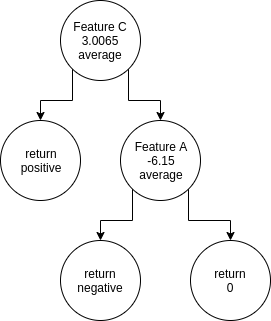
\includegraphics[scale=0.75]{Real_Tree.png}
\caption{Real Decision Tree}
\end{figure}

\end{document}
